\documentclass[nooutcomes]{ximera}
\usepackage{booktabs}
%% handout
%% space
%% newpage
%% numbers
%% nooutcomes

\renewcommand{\outcome}[1]{\marginpar{\null\vspace{2ex}\scriptsize\framebox{\parbox{0.75in}{\begin{raggedright}\textbf{P\arabic{problem} Outcome:} #1\end{raggedright}}}}}

\renewenvironment{freeResponse}{
\ifhandout\setbox0\vbox\bgroup\else
\begin{trivlist}\item[\hskip \labelsep\bfseries Solution:\hspace{2ex}]
\fi}
{\ifhandout\egroup\else
\end{trivlist}
\fi}

\newcommand{\RR}{\mathbb R}
\renewcommand{\d}{\,d}
\newcommand{\dd}[2][]{\frac{d #1}{d #2}}
\renewcommand{\l}{\ell}
\newcommand{\ddx}{\frac{d}{dx}}
\everymath{\displaystyle}
\newcommand{\dfn}{\textbf}
\newcommand{\eval}[1]{\bigg[ #1 \bigg]}


\title{Breakout Session 26 Solutions}

\begin{document}
\begin{abstract}
  % \textbf{A look back:} In a previous (April 19, 2016) Breakout Session you practiced applying the substitution rule to find indefinite integrals and evaluate definite integrals.

  % \textbf{Overview:} In this (April 21, 2016) last Breakout Session you'll practice applying definite integrals to compute net change.
\end{abstract}
\maketitle

% \section{Learning Outcomes}
% \label{section:learning-outcomes}
% The following outcomes are \emph{not an exhaustive} list of the skills you will need to develop and integrate for demonstration on quizzes and exams.
% This list is meant to be a starting point for conversation (with your Lecturer, Breakout Session Instructor, and fellow learners) for organizing your knowledge and monitoring the development of your skills.

% \begin{itemize}
%   \item
%     Given a velocity function, calculate displacement and distance traveled.

%   \item
%     Given a velocity function, find the position function.

%   \item
%     Given an acceleration function, find the velocity function.

%   \item
%     Understand the difference between displacement and distance traveled.

%   \item
%     Understand the relationship between position, velocity and acceleration.

%   \item
%     Calculate net change and future value.

%   \item
%     Understand how the net change and future value of a function are related to that function’s derivative.
% \end{itemize}
% \newpage

\begin{problem}
  \outcome{Given a velocity function, find the position function.}
  Consider an object moving along a line.
  The graph of the velocity, $v(t)$, of the object is shown in the figure below.
  \begin{image}
    \includegraphics[scale = 0.3]{Images/"Velocity small graph".png}
  \end{image}

  In the figure below, graph (the best you can) the position function, $s(t)$, given that $s(0) = 0$.
  \begin{image}
    \includegraphics[scale = 0.2]{Images/"Velocity large graph solution".png}
  \end{image}
\end{problem}

\begin{problem}
\outcome{Given a velocity function, calculate displacement and distance traveled.}
\outcome{Understand the difference between displacement and distance traveled.}
Solve the following word problems:

	\begin{enumerate}

	\item  The velocity function for a man walking along a straight road which runs east and west is given by
	$v(t) = -t^2 + 4t - 3$ feet per minute.

		\begin{enumerate}

		\item[i.]  Find the total displacement the man traveled from $2$ minutes to $6$ minutes (assume east is positive).
			\begin{freeResponse}
			The man's total displacement is given by $\int_2^6 v(t) \d t$.  So we compute:
				\begin{align*}
				\int_2^6 v(t) \d t &= \int_2^6 (-t^2 + 4t - 3) \d t  \\
				&= \eval{- \frac{1}{3} t^3 + 2t^2 - 3t}_2^6  \\
				&= (-72 + 72 - 18) - \left( - \frac{8}{3} + 8 - 6 \right)  \\
				&= \frac{8}{3} - 20 = - \frac{52}{3}.
				\end{align*}
			So the man's displacement is $\frac{52}{3}$ feet west of his original location.
			\end{freeResponse}

		\item[ii.]  Find the total distance the man traveled from $2$ minutes to $6$ minutes.
			\begin{freeResponse}
			First notice that $v(t) = -(t^2 - 4t + 3) = -(t-1)(t-3)$.  So we can see that
				\begin{align*}
				v(t) &> 0 \text{ when }  2 \leq t < 3.  \\
				v(t) &< 0 \text{ when } 3 < t \leq 6.
				\end{align*}
			Thus, the total distance that the man traveled from $2$ minutes to $6$ minutes is:
				\begin{align*}
				\int_2^6 \left| v(t) \right| \d t &= \int_2^3 \left| v(t) \right| \d t + \int_3^6 \left| v(t) \right| \d t  \\
				&= \int_2^3 v(t) \d t + \int_3^6 - v(t) \d t  \\
				&= \int_2^3 (-t^2 + 4t - 3) \d t - \int_3^6 (-t^2 + 4t - 3) \d t  \\
				&= \eval{- \frac{1}{3} t^3 + 2t^2 - 3t}_2^3 - \eval{- \frac{1}{3} t^3 + 2t^2 - 3t}_3^6  \\
				&= \left( (-9+18-9) - (- \frac{8}{3} + 8 - 6) \right) -  \\
				& \left( (-72+72-18)-(-9+18-9) \right)  \\
				&= \left(0 - 2 + \frac{8}{3} \right) - \left( -18 - 0 \right)  \\
				&=  16 + \frac{8}{3} = \frac{56}{3}.
				\end{align*}
			So, the total distance that the man traveled is $\frac{56}{3}$ feet.
			\end{freeResponse}

		\item[iii.]  Suppose that the man's position $2$ minutes into the trip is $5$ feet east of his mailbox.  What is his position (relative to his mailbox) at $6$ minutes.
			\begin{freeResponse}
			$s(6) = s(0) + \int_2^6 v(t) \d t = 5 + \left(- \frac{52}{3} \right) = - \frac{37}{3}. $

			So the man's position at $6$ minutes is $\frac{37}{3}$ feet west of his mailbox.
			\end{freeResponse}
		\end{enumerate}

	\item  Sammy the Snail sets up camp in the median of I-70 and, starting at noon and ending at 6pm, hikes back and forth along the highway.  He starts his hike at his campsite.  His velocity at time $t$ hours (after noon)  is given by $v(t)=(t-2)(t-5)$ inches per hour.  Find the total distance Sammy travelled on his hike.
		\begin{freeResponse}
		The total distance that Sammy travels is $\int_0^6 \left| v(t) \right| \d t$.
		The following picture indicates where $v(t)$ is positive and negative:
			\begin{image}
			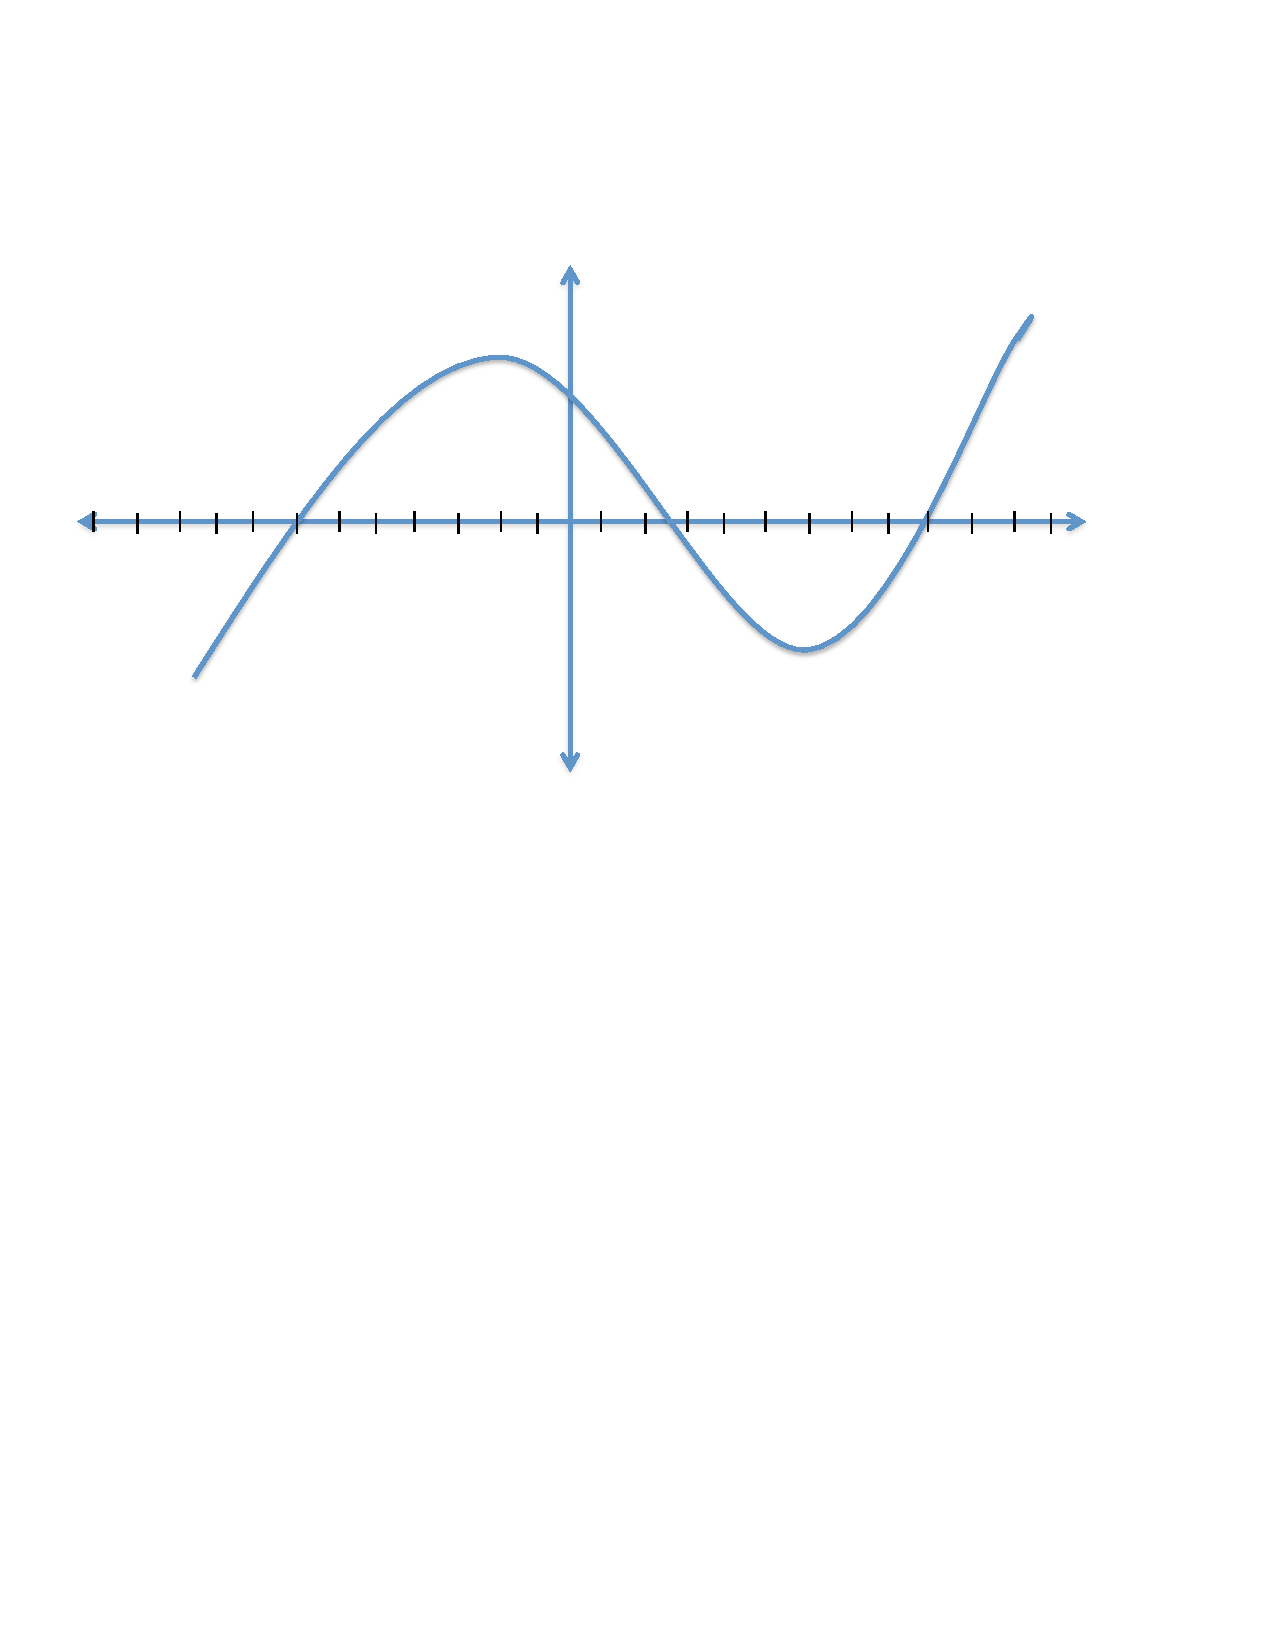
\includegraphics[trim= 170 400 250 290]{Images/Figure2.pdf}
			\end{image}
		So we compute:
			\begin{align*}
			\int_0^6 \left| v(t) \right| \d t &= \int_0^2 \left| v(t) \right| \d t + \int_2^5 \left| v(t) \right| \d t + \int_5^6 \left| v(t) \right| \d t  \\
			&= \int_0^2 v(t) \d t - \int_2^5 v(t) \d t + \int_5^6 v(t) \d t  \\
			&= \int_0^2 (t^2 - 7t + 10) \d t - \int_2^5 (t^2 - 7t + 10) \d t + \int_5^6 (t^2 - 7t + 10) \d t  \\
			&= \eval{\frac{1}{3}t^3-\frac{7}{2}t^2+10t}_0^2-\eval{\frac{1}{3}t^3-\frac{7}{2}t^2+10t}_2^5+\eval{\frac{1}{3}t^3-\frac{7}{2}t^2+10t}_5^6  \\
			&= \left( \left(\frac{8}{3}-14+20 \right)-0\right)-\left( \left( \frac{125}{3}-\frac{175}{2}+50 \right)-\left( \frac{8}{3}+6 \right) \right)+  \\
			&\left( \left( 72-126+60 \right) - \left( \frac{125}{3} - \frac{175}{2} + 50 \right) \right)  \\
			&= -82+175-78=15.
			\end{align*}
		So Sammy has traveled a distance of $15$ inches.
		\end{freeResponse}
	\end{enumerate}
\end{problem}

\begin{problem}
\outcome{Calculate net change and future value.}
\outcome{Understand how the net change and future value of a function are related to that function’s derivative.}
Assume that the {\it rate of change} (in dollars per day) of the price of shares of stock
in the WeSaySo Company (with $t$ in days) is modeled by the equation $r(t) = -3t^2+30t-63$
(note that this is technically a {\it discrete} function, but prices change so often with stocks that modeling this with a continuous function makes sense).
Assume also that the price of a share of stock on day $1$ (i.e., $t=1$) is $\$51$.
Answer the following questions:
	\begin{enumerate}

	\item  Find the rate of change of price at $t=5$.
		\begin{freeResponse}
		$r(5) = -3(25) + 30(5) - 63 = -75+150-63=12 \text{ dollars/day}$.
		\end{freeResponse}




	\item  Find the price of a share of stock at $t=5$.
		\begin{freeResponse}
		Let $p(t)$ denote the price of a share of stock at any time $t$.
		Then notice that $r(t) = p^\prime (t)$.
		We will first find $p(t)$ for general $t$, and then substitute $t=5$ to solve this problem.
			\begin{align*}
			p(t) &= \int_1^t r(s) \d s + p(1)  \\
			&= \int_1^t \left( -3s^2 + 30s - 63 \right) \d s + 51  \\
			&= \eval{ - s^3 + 15s^2 - 63s}_1^t + 51  \\
			&= \left( - t^3 + 15t^2 - 63t \right) - (-1+15-63) + 51  \\
			&= -t^3 + 15t^2 - 63t + 100.
			\end{align*}
		So, $p(5) = -125+375-315+100=35\$.$
		\end{freeResponse}




	\item  How fast is the rate of change of price changing at $t=5$?
		\begin{freeResponse}
		$r'(t) = -6t + 30$.  So, $r'(5) = -30+30=0$.
		\end{freeResponse}




	\item  How much did the price of a share of stock change in the first $6$ days (i.e., on $[1,6]$)?
		\begin{freeResponse}
		$p(6) - p(1) = (-216+540-378+100) - 51 = -5\$. $
		\end{freeResponse}




	\item  What was the greatest rate of change of price during the first $6$ days (i.e., on $[1,6]$)?
		\begin{freeResponse}
		This question wants us to maximize $r(t)$ on the closed interval $[1,6]$.
		So we need to find all critical points of $r(t)$ on $[1,6]$.
		$$ r'(t) = -6t+30:=0 \quad \Longrightarrow \quad t=5  $$
		Then, using the closed interval method, we simply plug $t=1,5,6$ into $r(t)$ and check which has the greatest output.
			\begin{align*}
			&r(1) = -3+30-63=-36  \\
			&r(5) = -75+150-63=12  \\
			&r(6) = -108+180-63=9.
			\end{align*}
		Thus, the greatest rate of change of price is $12$ dollars/day when $t=5$.
		\end{freeResponse}




	\item  What was the greatest price of a share of stock during the first $6$ days (i.e., on $[1,6]$)?
		\begin{freeResponse}
		This question wants us to maximize $p(t)$ on the closed interval $[1,6]$.
		So we need to find all critical points of $p(t)$ on $[1,6]$.
		But note that $p'(t) = r(t)$.  So critical points of $p(t)$ are just roots of $r(t)$.
		$$ r(t) = 0 $$
		$$ -3t^2+30t-63 = 0 $$
		$$ -3(t^2-10t+21)=0 $$
		$$ -3(t-3)(t-7) = 0 $$
		$$ t=3,7 \quad \Longrightarrow \quad t=3 $$
		since $7$ is not in the interval $[1,6]$.
		So we again use the closed interval method:
			\begin{align*}
			&p(1) = -1+15-63+100 = 51  \\
			&p(3) = -27 + 135 - 189 + 100 = 19  \\
			&p(6) = -216+540-378+100=46  \\
			\end{align*}
		Thus, the greatest price of the stock is $\$51$ when $t=1$.
		\end{freeResponse}
	\end{enumerate}
\end{problem}

\begin{problem}
\outcome{Calculate net change and future value.}
\outcome{Understand how the net change and future value of a function are related to that function’s derivative.}
Suppose that $r(t) = r_0 e^{-kt}$ (with $k>0$) is the rate at which a nation extracts oil.
The current rate of extraction is $r(0) = 10^7$ barrels/yr.
Also assume that the estimate of the total oil reserve (ie, the amount of oil remaining beneath the ground in this country) is $2 \times 10^9$ barrels.

	\begin{enumerate}

	\item  Find $Q(t)$, the total amount of oil extracted by the nation after $t$ years.
		\begin{freeResponse}
		$Q(t) = Q(0) + \int_0^t r(s) \d s$.  Note that $Q(0)=0$ since no oil will have been extracted in $0$ time.  So
			\begin{align*}
			Q(t) &= \int_0^t r(s) \d s  \\
			&= \int_0^t r_0 e^{-ks} \d s  \\
			&= - \frac{r_0}{k} \eval{e^{-ks}}_0^t  \\
			&= - \frac{r_0}{k} \left( e^{-kt} - 1 \right)  \\
			&= - \frac{1}{k} 10^7 \left(e^{-kt}-1 \right)  \\
			\end{align*}
		\end{freeResponse}

	\item  Evaluate $\lim_{t \to \infty} Q(t)$ and explain the meaning of this limit.
		\begin{freeResponse}
			\begin{align*}
			\lim_{t \to \infty} Q(t) &= \lim_{t \to \infty} - \frac{1}{k} 10^7 \left(e^{-kt}-1 \right)  \\
			&= - \frac{1}{k} 10^7 (0-1)  \\
			&= \frac{1}{k} 10^7.
			\end{align*}
		\end{freeResponse}

	\item  Find the minimum decay constant $k$ for which the total oil reserves will last forever.
		\begin{freeResponse}
		For the oil reserves to last forever, we need that
			\begin{align*}
			&\lim_{t \to \infty} Q(t) \leq 2 \times 10^9  \\
			 &\Longleftrightarrow \qquad \frac{1}{k} 10^7 \leq 2 \times 10^9  \\
			 &\Longleftrightarrow \qquad \frac{1}{k} \leq 2 \times 10^2 = 200  \\
			 &\Longleftrightarrow \qquad \frac{1}{200} \leq k.
			\end{align*}
		So the minimum value for $k$ is $\frac{1}{200}$.
		\end{freeResponse}

	\item  Suppose that the decay constant is half the minimum value found in part (c).

		\begin{freeResponse}
		First note that $k = \frac{1}{2} \cdot \frac{1}{200} = \frac{1}{400}$.
		We want to find the value of $t$ such that:
			\begin{equation*}
			Q(t) = 2 \times 10^9
			\end{equation*}
			\begin{equation*}
			- 400 \times 10^7 \left(e^{-\frac{1}{400}t}-1 \right) = 2 \times 10^9
			\end{equation*}
			\begin{equation*}
			\left(e^{-\frac{1}{400}t}-1 \right) = \frac{2 \times 10^9}{-400 \times 10^7} = - \frac{1}{2}
			\end{equation*}
			\begin{equation*}
			e^{-\frac{1}{400}t} = \frac{1}{2}
			\end{equation*}
			\begin{equation*}
			-\frac{1}{400}t=\ln \left(\frac{1}{2} \right) = -\ln(2)
			\end{equation*}
			\begin{equation*}
			t = 400 \ln(2) \approx 277.259 \text{ years}.
			\end{equation*}
		\end{freeResponse}
	\end{enumerate}
\end{problem}

\section{Extra Problems for Personal Practice}
\begin{problem}
  A bug is moving down the curve $y = \frac{8}{x}$, starting at the point $A$ (see figure).
  Its $x$-coordinate is increasing at the rate of 6 cm/min.
  \begin{image}
    \includegraphics[scale = 0.3]{Images/"Bug on parabola".png}
  \end{image}
  \begin{itemize}
    \item[(i)]
      At what rate is the bug's $y$-coordinate changing when $x = 4$?
      \begin{freeResponse}
        We have
        \begin{align*}
          y = \frac{8}{x} &\implies \frac{\d y}{\d t} = \frac{-8}{x^2} \frac{\d x}{\d t} \\
          &= \implies \frac{\d y}{\d t} = \frac{-8}{4^2} \cdot 6 = -3
        \end{align*}
      \end{freeResponse}

    \item[(ii)]
      At what rate is \underline{the distance} between the bug and the origin changing when $x = 4$?
      \begin{freeResponse}
        The distance between the origin and the bug is given by
        \[
          \text{s} = \sqrt{(x- 0)^2 + (y - 0)^2} = \sqrt{x^2 + y^2}
        \]
        Therefore
        \begin{align*}
          \frac{\d s}{\d t} &= \frac{1}{2\sqrt{x^2+y^2}}\cdot \left(2 x \cdot \frac{dx}{dt} + 2y \cdot\frac{dy}{dt}\right) \\
          &= \implies \frac{ds}{dt} = \frac{x (dx/dt) + y (dy/dt)}{\sqrt{x^2+y^2}}
        \end{align*}

        When $x = 4$ we have $y = 8/4 = 2$.
        Hence
        \[
          \frac{\d s}{\d t} = \frac{4 \cdot 6 + 2 \cdot (-3)}{\sqrt{4^2 + 2^2}} = \frac{18}{\sqrt{20}}.
        \]
      \end{freeResponse}

    \item[(iii)]
      For what value of $x$ is the bug closest to the origin?
      Justify your answer.
      \begin{freeResponse}
        When minimizing distance, it's better to work with the square of the distance instead of distance directly.

        Finding objective function:
        \begin{align*}
          \text{distance}^2 &= x^2 + y^2 \\
          &\implies \text{distance}^2 = x^2 + (8/x)^2\\
          &\implies f(x) =  x^2 + (8/x)^2
        \end{align*}

        Constraint on objective function:
        \[
          \text{Domain}(f) = [1, 8]
        \]

        Finding critical point(s):
        \begin{align*}
          f'(x) = 2x + \frac{-128}{x^3} &\implies f'(x) = 0 \\
          &\implies 2x - \frac{128}{x^3} = 0 \\
          &\implies 2x = \frac{128}{x^3} \\
          &\implies x^4 = 64 \\
          &\implies x = 2\sqrt{2}
        \end{align*}

        Since we only have one interior point, to verify the absolute minimum occurs at $x = 2\sqrt{2}$ we examine the sign of $f'$ near $x = 2\sqrt{2}$:
        \begin{image}
          \includegraphics[scale = 0.3]{Images/"Sign of first derivative".png}
        \end{image}
        Hence there is a local minimum at $x = 2\sqrt{2}$.
        Since there is only one local extrema and $f$ is continuous on $[1, 8]$ we have
        \begin{align*}
          \mbox{local minimum at $x = 2\sqrt{2}$} \implies \mbox{absolute minimum at $x = 2\sqrt{2}$}
        \end{align*}
      \end{freeResponse}
  \end{itemize}
\end{problem}

\end{document}
%
